
%(BEGIN_QUESTION)
% Copyright 2014, Tony R. Kuphaldt, released under the Creative Commons Attribution License (v 1.0)
% This means you may do almost anything with this work of mine, so long as you give me proper credit

A set of three 50/51 protective relays protects a feeder line supplying power to a number of different industrial loads at 13.8 kV.  After operating for several years without incident, one day the circuit breaker trips.  One of the three relay's target shows ``51'' but not ``50'' following the breaker trip.  A thorough inspection and test of the feeder line reveals no faults along the power line itself (e.g. no tree branches touching, no cracked insulators, etc.):

$$\includegraphics[width=15.5cm]{i03107x01.eps}$$

Identify the likelihood of each specified fault in this system, to explain why the breaker tripped despite there being no fault in the feeder.  Consider each fault one at a time (i.e. no coincidental faults), determining whether or not each fault could independently account for {\it all} observations and symptoms in this circuit.

% No blank lines allowed between lines of an \halign structure!
% I use comments (%) instead, so that TeX doesn't choke.

$$\vbox{\offinterlineskip
\halign{\strut
\vrule \quad\hfil # \ \hfil & 
\vrule \quad\hfil # \ \hfil & 
\vrule \quad\hfil # \ \hfil \vrule \cr
\noalign{\hrule}
%
% First row
{\bf Fault} & {\bf Possible} & {\bf Impossible} \cr
%
\noalign{\hrule}
%
% Another row
125 VDC station power supply dead &  &  \cr
%
\noalign{\hrule}
%
% Another row
CT failed open &  &  \cr
%
\noalign{\hrule}
%
% Another row
CT failed shorted &  &  \cr
%
\noalign{\hrule}
%
% Another row
Mild, prolonged overload condition &  &  \cr
%
\noalign{\hrule}
%
% Another row
Bolted fault at one of the loads &  &  \cr
%
\noalign{\hrule}
} % End of \halign 
}$$ % End of \vbox

\underbar{file i03107}
%(END_QUESTION)





%(BEGIN_ANSWER)

% No blank lines allowed between lines of an \halign structure!
% I use comments (%) instead, so that TeX doesn't choke.

$$\vbox{\offinterlineskip
\halign{\strut
\vrule \quad\hfil # \ \hfil & 
\vrule \quad\hfil # \ \hfil & 
\vrule \quad\hfil # \ \hfil \vrule \cr
\noalign{\hrule}
%
% First row
{\bf Fault} & {\bf Possible} & {\bf Impossible} \cr
%
\noalign{\hrule}
%
% Another row
125 VDC station power supply dead &  & $\surd$ \cr
%
\noalign{\hrule}
%
% Another row
CT failed open &  & $\surd$ \cr
%
\noalign{\hrule}
%
% Another row
CT failed shorted &  & $\surd$ \cr
%
\noalign{\hrule}
%
% Another row
Mild, prolonged overload condition & $\surd$ &  \cr
%
\noalign{\hrule}
%
% Another row
Bolted fault at one of the loads &  & $\surd$ \cr
%
\noalign{\hrule}
} % End of \halign 
}$$ % End of \vbox

%(END_ANSWER)





%(BEGIN_NOTES)

{\bf This question is intended for exams only and not worksheets!}.

%(END_NOTES)



